% IEEE conference-format manuscript. Compile: pdflatex paper.tex (twice). Requires IEEEtran.cls (standard in TeX Live / Overleaf).
% The bibliography is generated from build_refs.py (single source of truth, also writes references.bib).
\documentclass[conference]{IEEEtran}
\usepackage{graphicx}
\usepackage{booktabs}
\usepackage{amsmath}
\usepackage{cite}
\usepackage{url}
\usepackage[T1]{fontenc}
\graphicspath{{../../results/figures/}}
\newcommand{\tabsize}{\footnotesize}

\begin{document}

\title{Does Dimensionality Reduction Help Classical Intrusion Detection? A Leakage-Controlled Comparison of Original Features, PCA and Kernel PCA on a CIC-IDS2017 Sample}

\author{\IEEEauthorblockN{[Author One]}
\IEEEauthorblockA{[Department], [Institution]\\
{[City, Country]}\\
{[email]}}
\and
\IEEEauthorblockN{[Author Two]}
\IEEEauthorblockA{[Department], [Institution]\\
{[City, Country]}\\
{[email]}}}

\maketitle

\begin{abstract}
Kernel PCA (KPCA) is often paired with classical classifiers for network intrusion detection, but reported gains are usually measured with accuracy on a single split and without a no-reduction baseline. We compare three feature spaces---the original 78 flow features, PCA, and KPCA with linear, RBF and cosine kernels (5--30 components)---across five classifiers (logistic regression, $k$-NN, SVM, decision tree, random forest) on a 1{,}000-record stratified sample of CIC-IDS2017 (11 classes, 71.8\% benign). Imputation, scaling and reduction are fitted on training folds only; evaluation uses repeated stratified 5-fold cross-validation (15 folds) with accuracy, macro-F1, balanced accuracy and MCC, paired Wilcoxon tests with Holm correction, and a runtime/memory benchmark. The strongest model was a random forest on the \emph{original} features (accuracy $0.952\pm0.010$, macro-F1 $0.722\pm0.058$, MCC $0.894\pm0.022$; majority-class baseline: accuracy 0.718, macro-F1 0.076). No PCA or KPCA setting improved on the original features for logistic regression, decision tree or random forest, and $k$-NN showed no significant difference; the exception was an RBF-kernel SVM, whose macro-F1 rose from 0.39 to 0.51 with 30-component cosine KPCA. Linear KPCA reproduced PCA, as theory predicts. KPCA raised fitting time roughly tenfold and peak traced memory from 1.7 to 11.7\,MB at 800 training records, with memory growing quadratically in sample size. Results come from one small sample of one dataset; they do not establish generalization to unseen traffic.
\end{abstract}

\begin{IEEEkeywords}
network intrusion detection, kernel PCA, dimensionality reduction, CIC-IDS2017, class imbalance, empirical comparison
\end{IEEEkeywords}

\section{Introduction}
Machine-learning network intrusion detection systems (NIDS) are commonly developed and compared on public flow datasets \cite{ring2019}, of which CIC-IDS2017 \cite{sharafaldin2018} is one of the most used. Its flow records carry 78 numeric features, which motivates dimensionality reduction as a way to cut training cost and possibly improve generalization. Linear PCA and auto-encoders have been applied to CIC-IDS2017 \cite{abdulhammed2019}, and Kernel PCA (KPCA) \cite{scholkopf1998}, which performs PCA in an implicit nonlinear feature space, has been combined with SVMs for intrusion detection \cite{kuang2014}.

Three methodological issues make such comparisons hard to interpret. First, CIC-IDS2017 is class-imbalanced and, in its original form, contains labelling and flow-construction problems \cite{engelen2021,panigrahi2018}, so accuracy can be dominated by the benign majority. Second, common pitfalls in security-oriented machine learning---including evaluation set-ups that overstate real performance---are widespread \cite{arp2022}. Third, many studies omit the simplest baseline, the original feature space, so a benefit of the reduction is assumed rather than measured.

\textbf{Research questions.} We ask: \textbf{RQ1} how does reduction affect multi-class detection performance; \textbf{RQ2} does KPCA beat the original space or conventional PCA; \textbf{RQ3} how do kernel, component count and classifier interact; \textbf{RQ4} what does the reduction cost in time and memory; \textbf{RQ5} how stable are the conclusions under repeated, class-aware validation and smaller training sets.

\textbf{Contributions.} (i) A leakage-controlled, reproducible comparison of original features, PCA and three KPCA kernels over five classical classifiers, including a majority-class baseline. (ii) A class-aware analysis (macro-F1, balanced accuracy, MCC, per-class recall) showing how much accuracy overstates detection quality on this data. (iii) Paired statistical tests of the comparisons that matter, with an explicit caveat on their independence. (iv) A runtime and memory measurement of KPCA against PCA. We do not propose a new algorithm. All code, raw per-fold results and scripts are in the project repository.

\section{Related Work}
\textit{Datasets.} Ring et al.\ survey network-based intrusion datasets and the properties that determine their suitability for evaluation scenarios \cite{ring2019}. CIC-IDS2017 was introduced by Sharafaldin et al.\ \cite{sharafaldin2018}. Engelen et al.\ report problems in it: ``TCP appendix'' artefact flows (about a quarter of all flows), attack attempts labelled as attacks although they contain no malicious payload, and feature-extraction flaws that enable shortcut learning; they released a corrected version \cite{engelen2021}. Panigrahi and Borah likewise describe shortcomings of the dataset and propose a combined dataset \cite{panigrahi2018}. We use the \emph{original} labelled flows, so absolute scores here may partly reflect such artefacts.

\textit{Dimensionality reduction for NIDS.} Abdulhammed et al.\ apply an auto-encoder and PCA to CIC-IDS2017, reducing the feature count from 81 to 10 while reporting 99.6\% accuracy with random forest and other classifiers \cite{abdulhammed2019}. Kuang et al.\ propose a hybrid of KPCA, an SVM and a genetic algorithm for intrusion detection \cite{kuang2014}. This section is not a systematic survey; it positions the present study rather than claiming to cover the literature.

\textit{Evaluation practice.} Arp et al.\ document recurring methodological pitfalls in machine learning for security that lead to unrealistic performance \cite{arp2022}, and Apruzzese et al.\ show that cross-dataset evaluation of NIDS reveals behaviour that single-dataset testing hides \cite{apruzzese2022}. Motivated by this, we (a) fit every data-dependent step on training folds only, (b) report class-aware metrics next to accuracy, (c) include trivial and no-reduction baselines, and (d) state plainly what our sample cannot show.

\section{Dataset and Preprocessing}
\textbf{Data.} The study uses the cached 1{,}000-record stratified sample shipped with the project (\texttt{data/sample.npz}), drawn from the Tuesday, Wednesday and Thursday-morning files of CIC-IDS2017 (1{,}308{,}978 flows according to the project documentation; the raw files were not available in the authoring environment, so this count was not recomputed). The sample has 78 numeric features, 11 classes and at least 10 records per class (Table~\ref{tab:classes}); 718 records (71.8\%) are benign. Ten features are constant in the sample. The sample was drawn by the project's \texttt{prepare\_data.py}.

\textbf{A leakage caveat in the cached sample.} The project's original script mean-imputed missing values using all flows \emph{before} sampling. The imputed values in the cached sample therefore carry information from the full dataset. We could not undo this without the raw files; the pipeline below still performs imputation inside each training fold (a no-op on this sample), and the raw-data script \texttt{prepare\_raw.py} removes the issue for future runs. The practical effect is likely small (a mean over 1.3\,M flows) but is not measured.

\begin{table}[t]
\caption{Class distribution of the 1{,}000-record sample.}\label{tab:classes}
\centering\tabsize
\begin{tabular}{lrr}
\toprule
Class & Records & \% \\
\midrule
BENIGN & 718 & 71.8 \\
DoS GoldenEye & 17 & 1.7 \\
DoS Hulk & 167 & 16.7 \\
DoS Slowhttptest & 14 & 1.4 \\
DoS slowloris & 14 & 1.4 \\
FTP-Patator & 15 & 1.5 \\
Heartbleed & 10 & 1.0 \\
SSH-Patator & 14 & 1.4 \\
Web Brute Force & 11 & 1.1 \\
Web Sql Injection & 10 & 1.0 \\
Web XSS & 10 & 1.0 \\
\bottomrule
\end{tabular}

\end{table}

\section{Methodology}
\textbf{Pipeline.} Fig.~\ref{fig:pipe} shows the protocol. Within each training fold we fit a mean imputer and a standard scaler, then the dimensionality reducer; test folds are only transformed. Feature spaces are: \emph{original} (78 standardised features); \emph{PCA}; and \emph{KPCA} with linear, RBF (scikit-learn default $\gamma=1/78$) and cosine kernels \cite{scholkopf1998}, each with $n\in\{5,10,15,20,30\}$ components. The original design tied kernel and component count (RBF--5, linear--10, cosine--15); here they are crossed so the two effects can be separated. The reducer is fitted once per fold and shared by all classifiers, which is equivalent to fitting it inside each pipeline because it is deterministic (verified by a unit test against a scikit-learn \texttt{Pipeline}).

\begin{figure*}[t]\centering
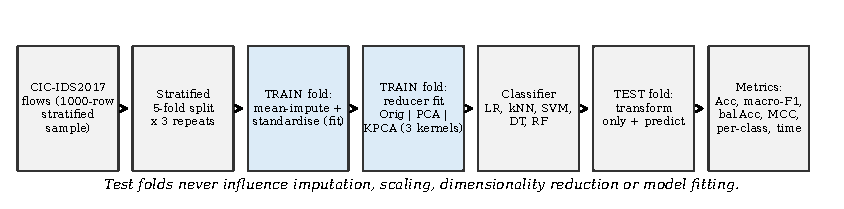
\includegraphics[width=\textwidth]{fig1_pipeline.pdf}
\caption{Experimental pipeline. All data-dependent preprocessing and reduction is fitted on the training fold only.}\label{fig:pipe}
\end{figure*}

\textbf{Classifiers.} Logistic regression (L2, lbfgs), $k$-NN with $k=5$ \cite{cover1967}, an SVM with RBF kernel, $C=1$ and $\gamma$=``scale'' \cite{cortes1995}, a decision tree with entropy criterion \cite{quinlan1986}, and a random forest with 100 trees \cite{breiman2001}, using scikit-learn \cite{pedregosa2011}. Hyper-parameters are fixed to the project's original values and \emph{not} tuned. Each classifier except $k$-NN is also run with \texttt{class\_weight=balanced}. A majority-class classifier is the trivial baseline. Resampling (e.g.\ SMOTE) is not used: some classes have only 7--8 training records per fold, too few for meaningful synthetic interpolation.

\textbf{Validation.} Repeated stratified 5-fold cross-validation, 3 repeats (15 folds), seed 42; every method sees identical folds, giving paired observations. Rare classes have 2--3 test records per fold, so per-fold macro-F1 is noisy; we therefore report means and standard deviations over the 15 folds.

\textbf{Metrics.} Accuracy; macro-precision, macro-recall and macro-F1; weighted-F1; balanced accuracy; and the multi-class Matthews correlation coefficient (MCC) \cite{chicco2020}. \textbf{Macro-F1 is the primary model-selection criterion}, chosen before the runs because it weights all 11 classes equally. Per-class results and the confusion matrix use pooled out-of-fold predictions of the first repeat.

\textbf{Statistics.} For each classifier we compare feature spaces at a matched $n=10$ with two-sided Wilcoxon signed-rank tests on the 15 paired macro-F1 values, Holm-corrected over the 30 comparisons, with the matched-pairs rank-biserial correlation $r$ as effect size, and Friedman omnibus tests \cite{demsar2006}. Because cross-validation folds share training data, the 15 differences are not independent and the $p$-values are optimistic \cite{nadeau2003}; we use them for screening, not as proof. A second family compares the original space with each classifier's best reduced space (selected on the same folds, which favours the reduced space).

\textbf{Cost.} A serial benchmark (no parallel workers) records training and inference time (median of 5 repetitions, one fold split) and peak memory from Python's \texttt{tracemalloc}, measured in a separate pass. Native allocations inside compiled code are not traced, so memory figures are lower bounds that are most reliable for comparing the reducers.

\section{Experimental Setup}
All experiments ran on a 2-vCPU Intel Xeon @ 2.10\,GHz virtual machine with 7\,GB RAM (Linux, Python 3.13.16, scikit-learn 1.9.1, NumPy 2.5.3, SciPy 1.18.1). The main grid contains 21 feature spaces $\times$ 5 classifiers $\times$ 2 weighting schemes (plus the baseline) $\times$ 15 folds = 2{,}850 fits, run with two parallel workers; timings in Table~\ref{tab:rt} come from the separate serial benchmark. A second run repeats the five main spaces at $n=10$ with 10 random stratified splits at test fractions 0.2, 0.4 and 0.6 (training size 800, 600, 400) to examine sensitivity to training-set size. This is \emph{not} a temporal or cross-dataset split: the cached sample has no timestamps or day labels.

\section{Results}
\subsection{Original-feature baseline and the cost of reading accuracy alone}
Predicting the majority class gives accuracy 0.718 but macro-F1 0.076 and MCC 0.000. The random forest on original features reaches accuracy $0.952\pm0.010$ but macro-F1 $0.722\pm0.058$ (weighted-F1 0.947, balanced accuracy 0.717, MCC $0.894\pm0.022$): the gap between accuracy and macro-F1 comes from rare classes. Per class (Table~\ref{tab:perclass}), benign, DoS Hulk, FTP-Patator, SSH-Patator and Heartbleed are detected with F1 $\ge$ 0.96, whereas the three web attacks (brute force, SQL injection, XSS) obtain F1 between 0.21 and 0.50 on only 10--11 records each, and slow-DoS recalls are 0.57--0.71. These are the weak points that accuracy hides (Figs.~\ref{fig:acc} and~\ref{fig:f1}).

\begin{table}[t]
\caption{Per-class results of the selected model (RF, original features), pooled out-of-fold predictions, repeat 1.}\label{tab:perclass}
\centering\tabsize
\begin{tabular}{lrrrr}
\toprule
Class & Precision & Recall & F1 & Support \\
\midrule
BENIGN & 0.965 & 0.992 & 0.978 & 718 \\
DoS GoldenEye & 0.875 & 0.824 & 0.848 & 17 \\
DoS Hulk & 0.975 & 0.952 & 0.964 & 167 \\
DoS Slowhttptest & 1.000 & 0.571 & 0.727 & 14 \\
DoS slowloris & 0.909 & 0.714 & 0.800 & 14 \\
FTP-Patator & 1.000 & 1.000 & 1.000 & 15 \\
Heartbleed & 1.000 & 1.000 & 1.000 & 10 \\
SSH-Patator & 0.933 & 1.000 & 0.966 & 14 \\
Web Brute Force & 0.250 & 0.182 & 0.211 & 11 \\
Web Sql Injection & 0.667 & 0.400 & 0.500 & 10 \\
Web XSS & 0.400 & 0.400 & 0.400 & 10 \\
\bottomrule
\end{tabular}

\end{table}

\begin{figure*}[t]\centering
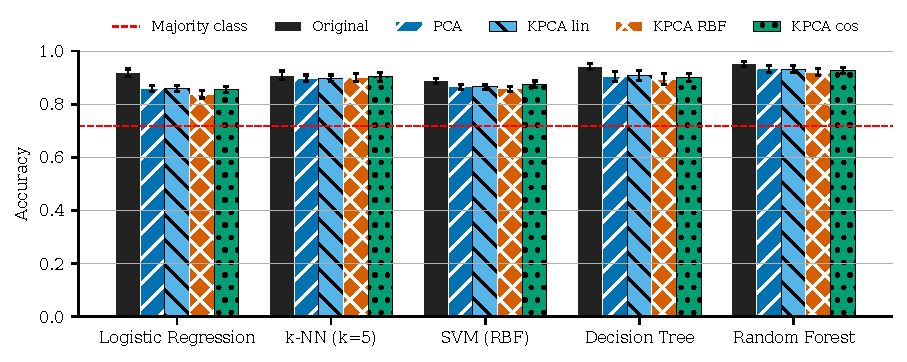
\includegraphics[width=\textwidth]{fig3_accuracy.pdf}\\[2pt]
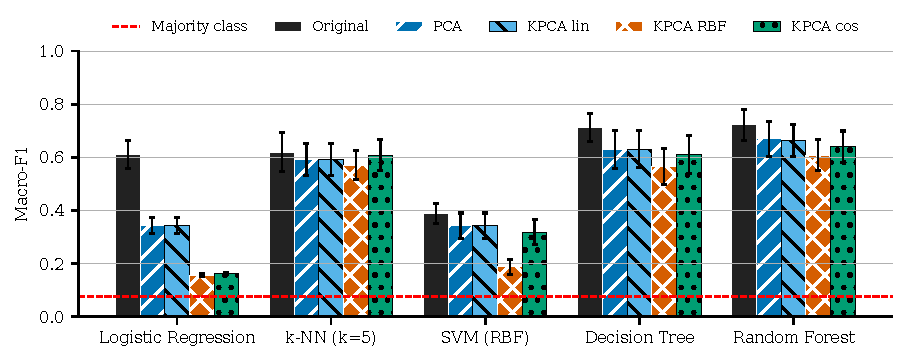
\includegraphics[width=\textwidth]{fig4_macro_f1.pdf}
\caption{Accuracy (top) and macro-F1 (bottom), mean $\pm$ std over 15 folds, 10 components for reduced spaces, standard class weights. Dashed line: majority-class classifier. Axes start at zero.}\label{fig:acc}\label{fig:f1}
\end{figure*}

\subsection{Original space versus PCA versus Kernel PCA}
Table~\ref{tab:n10} and Fig.~\ref{fig:f1} compare spaces at $n=10$. For every classifier, the original space has the highest or (for $k$-NN) statistically indistinguishable macro-F1. Of the 30 Holm-corrected comparisons, 17 were significant; in every significant comparison involving the original space it was the better one, and RBF-KPCA was significantly worse than PCA for LR, SVM, DT and RF. Cosine KPCA differed significantly from PCA only for logistic regression (where PCA was better). Against each classifier's \emph{best} reduced space (Table~\ref{tab:best}), the original features still won significantly for LR, DT and RF (Holm $p<0.01$, large effects); $k$-NN showed no difference; and the SVM was the single clear case where reduction helped: cosine KPCA with 30 components raised macro-F1 from 0.388 to 0.510 ($p_\mathrm{Holm}=0.0003$, better in all 15 folds). That comparison is selected on the same folds and therefore optimistic, and the SVM baseline itself is weak (class weighting alone lifts it to 0.546), so we read it as a sign that default-$\gamma$ RBF-SVM is poorly matched to heavy-tailed standardised features rather than as a general benefit of KPCA.

\begin{table*}[t]
\caption{Accuracy / macro-F1 ($\pm$ std over 15 folds) at 10 components (original = 78 features), standard class weights.}\label{tab:n10}
\centering\tabsize
\begin{tabular}{lccccc}
\toprule
Space & LR & KNN & SVM & DT & RF \\
\midrule
Original (78) & 0.919 / 0.612$\pm$0.052 & 0.909 / 0.620$\pm$0.074 & 0.888 / 0.388$\pm$0.037 & 0.943 / 0.713$\pm$0.054 & 0.952 / 0.722$\pm$0.058 \\
PCA-10 & 0.859 / 0.344$\pm$0.030 & 0.897 / 0.591$\pm$0.059 & 0.866 / 0.342$\pm$0.048 & 0.905 / 0.630$\pm$0.072 & 0.934 / 0.669$\pm$0.065 \\
KPCA-lin-10 & 0.859 / 0.344$\pm$0.030 & 0.897 / 0.591$\pm$0.059 & 0.866 / 0.342$\pm$0.048 & 0.908 / 0.631$\pm$0.069 & 0.933 / 0.664$\pm$0.060 \\
KPCA-RBF-10 & 0.837 / 0.156$\pm$0.006 & 0.900 / 0.571$\pm$0.056 & 0.858 / 0.187$\pm$0.029 & 0.894 / 0.565$\pm$0.067 & 0.921 / 0.608$\pm$0.058 \\
KPCA-cos-10 & 0.855 / 0.163$\pm$0.004 & 0.903 / 0.608$\pm$0.059 & 0.875 / 0.319$\pm$0.046 & 0.902 / 0.610$\pm$0.072 & 0.927 / 0.640$\pm$0.059 \\
\bottomrule
\end{tabular}

\end{table*}

\begin{table}[t]
\caption{Original features versus each classifier's best reduced space (Wilcoxon, Holm-corrected). Positive $\Delta$: original better.}\label{tab:best}
\centering\tabsize
\resizebox{\columnwidth}{!}{\begin{tabular}{llrrrrr}
\toprule
Clf & Best reduced space & F1 orig & F1 reduced & $\Delta$F1 (orig-red.) & $p_{Holm}$ & $r$ \\
\midrule
LR & kpca-linear-30 & 0.612 & 0.569 & 0.043 & 0.000 & 1.000 \\
KNN & kpca-cosine-15 & 0.620 & 0.628 & -0.008 & 0.679 & -0.133 \\
SVM & kpca-cosine-30 & 0.388 & 0.510 & -0.122 & 0.000 & -1.000 \\
DT & kpca-cosine-15 & 0.713 & 0.632 & 0.082 & 0.001 & 0.933 \\
RF & pca-10 & 0.722 & 0.669 & 0.053 & 0.002 & 0.981 \\
\bottomrule
\end{tabular}
}
\end{table}

\subsection{Kernel and component count}
Linear KPCA is mathematically equivalent to PCA on centred data; the two matched to within numerical noise (macro-F1 differences $\le0.011$ over all classifier and component settings; Fig.~\ref{fig:comp}). Hence the original project's best result (random forest, ``linear KPCA, 10 components'') is a PCA result, not evidence for a nonlinear kernel. Component count mattered mainly for logistic regression (macro-F1 0.28 at 5 components to 0.57 at 30 with PCA, still below 0.61 on the original features) and for the cosine-KPCA SVM; for $k$-NN, DT and RF the curves are flat (Fig.~\ref{fig:comp}). RBF-KPCA with the default $\gamma$ was the weakest kernel for most classifiers; we did not tune $\gamma$, so this is a statement about the default, not about RBF-KPCA in general.

\begin{figure*}[t]\centering
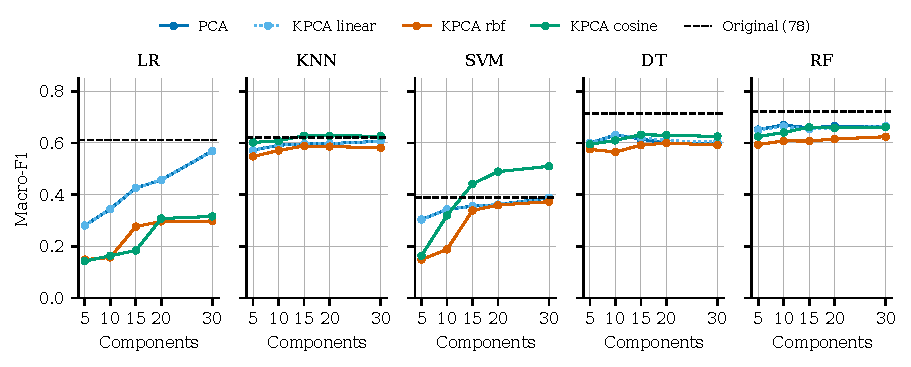
\includegraphics[width=\textwidth]{fig6_components_vs_f1.pdf}
\caption{Macro-F1 versus number of components for PCA and three KPCA kernels; dashed line: original 78 features.}\label{fig:comp}
\end{figure*}

\subsection{Class weighting}
Balanced class weights raised balanced accuracy for LR (0.638 $\to$ 0.778) and SVM (0.358 $\to$ 0.720) on the original features, but macro-F1 improved only for LR (0.612 $\to$ 0.630) and SVM (0.388 $\to$ 0.546) and \emph{fell} for DT and RF (0.713 $\to$ 0.702, 0.722 $\to$ 0.687). The best macro-F1 overall nonetheless remained the unweighted random forest, so the selected model does not depend on this choice.

\subsection{Computational cost}
Table~\ref{tab:rt} summarises the serial benchmark at 800 training / 200 test records. KPCA fitting took about 0.09--0.12\,s against 0.01\,s for PCA, increased decision-tree training time from 0.016\,s to roughly 0.09--0.10\,s and random-forest training from 0.21\,s to 0.36--0.38\,s, and roughly doubled random-forest inference time (0.007\,s to 0.014--0.016\,s per 200 records), since each new sample needs kernel evaluations against all training records. Peak traced memory was 11.7\,MB for KPCA against 1.7\,MB for PCA or no reduction. Over $n=400,600,800,1000$ KPCA fit time and memory grew roughly quadratically (3.1, 6.4, 11.0, 16.8\,MB; $\approx n^2$), as expected for an $n\times n$ kernel matrix. Extrapolating the memory formula, a kernel matrix for all 1.3\,M source flows would need on the order of 14\,TB of 64-bit floats, so exact KPCA cannot be applied to the full dataset without approximation (not tested here). Absolute times are sub-second on a shared 2-vCPU machine; differences below roughly a factor of two should not be over-interpreted. We make no real-time claim: only batch latencies on this machine were measured.

\begin{table}[t]
\caption{Serial runtime and traced peak memory (800 train / 200 test), median of 5.}\label{tab:rt}
\centering\tabsize
\resizebox{\columnwidth}{!}{\begin{tabular}{lrrrrr}
\toprule
Space & Reducer fit (s) & DT train (s) & RF train (s) & RF infer. (s) & Peak mem (MB) \\
\midrule
Original (78) & 0.000 & 0.018 & 0.190 & 0.007 & 1.687 \\
PCA-10 & 0.010 & 0.016 & 0.208 & 0.007 & 1.686 \\
KPCA-lin-10 & 0.104 & 0.085 & 0.370 & 0.014 & 11.750 \\
KPCA-RBF-10 & 0.119 & 0.100 & 0.359 & 0.015 & 11.750 \\
KPCA-cos-10 & 0.091 & 0.098 & 0.375 & 0.016 & 11.750 \\
\bottomrule
\end{tabular}
}
\end{table}

\subsection{Sensitivity to training-set size}
Fig.~\ref{fig:size} shows macro-F1 at 400, 600 and 800 training records over 10 random splits each. For LR, SVM, DT and RF the original space had the highest mean macro-F1 at every size, so the ranking in Table~\ref{tab:n10} is not an artefact of one training size; for $k$-NN the spaces overlap within one standard deviation. This is a stability check within the same sample and distribution, not a test of generalization to unseen traffic.

\begin{figure*}[t]\centering
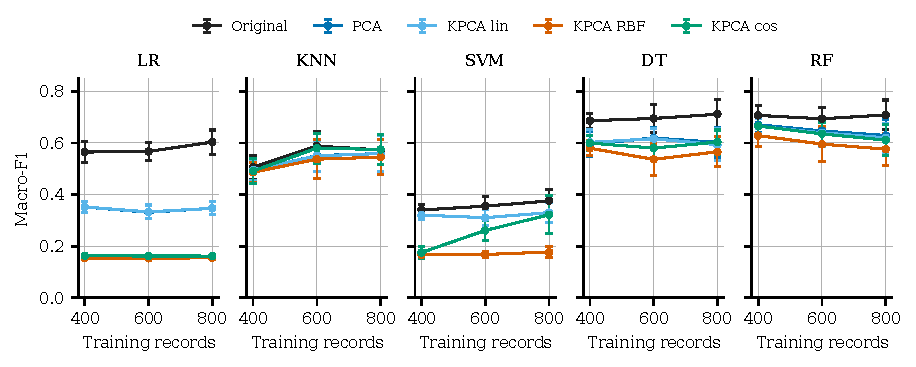
\includegraphics[width=\textwidth]{fig9_training_size.pdf}
\caption{Macro-F1 versus training-set size (random stratified splits, 10 per size, mean $\pm$ std); 10 components for reduced spaces.}\label{fig:size}
\end{figure*}

\section{Discussion}
\textbf{Answers to the research questions.} RQ1/RQ2: on this sample, reducing 78 standardised features to 5--30 PCA or KPCA components did not improve and usually lowered macro-F1; the one robust gain was for the RBF-SVM with cosine KPCA. RQ3: kernel mattered more than component count for most classifiers, with RBF (default $\gamma$) worst; linear KPCA equals PCA. RQ4: KPCA multiplied fitting time about tenfold and memory about sevenfold at $n=800$ and scales quadratically, with no accuracy benefit to offset it for four of five classifiers. RQ5: orderings were stable across repeated folds and training sizes within the sample.

\textbf{Why accuracy misleads.} The benign class makes up 71.8\% of records, so the trivial baseline already has accuracy 0.718; high accuracies of 0.93--0.95 for the best models correspond to macro-F1 of 0.66--0.72. The original project reported weighted-F1 and accuracy from single splits, which hide rare-class failure and cannot show whether a difference of a point or two is noise (the standard deviation of macro-F1 across folds is 0.05--0.07).

\textbf{Plausible but untested explanations.} Tree ensembles are insensitive to monotone feature scaling and can exploit individual informative features; projecting onto a few leading components may discard low-variance but discriminative directions. Heavy-tailed flow features also make variance-based reduction and the default RBF width poorly matched. These are hypotheses we did not test (e.g.\ with tuned $\gamma$, robust scaling, or supervised reduction).

\section{Threats to Validity and Limitations}
\textbf{Sample size and imbalance.} The sample has 1{,}000 records; nine of the ten attack classes have only 10--17 records, so per-class estimates are very uncertain and the macro-F1 is sensitive to a few records. \textbf{Population.} Only three of the eight CIC-IDS2017 files were sampled, one sample was used, and each attack family occurs on a single day in those files. \textbf{Dataset quality.} The original dataset contains known labelling and feature artefacts \cite{engelen2021}, which may inflate or distort scores. \textbf{Residual leakage.} The cached sample's imputation used full-data means (Section~III). \textbf{Selection and inference.} The model was selected on the same cross-validation that produced the reported scores, so its scores are optimistic; no external hold-out was possible with 10-record classes. Repeated-CV tests are not independent \cite{nadeau2003}. \textbf{Tuning.} Hyper-parameters, including the RBF $\gamma$, were fixed, not tuned. \textbf{Generalization.} No temporal, cross-day or cross-dataset evaluation was performed \cite{apruzzese2022}; conclusions apply to random splits of this sample. \textbf{Cost.} Memory is a traced lower bound; timings are from one virtual machine. We therefore make no claim of state-of-the-art, real-time or deployment-ready performance.

\section{Conclusion}
On a 1{,}000-record sample of CIC-IDS2017 and under leakage-controlled repeated cross-validation, a random forest on the original 78 features gave the best class-aware performance (macro-F1 $0.722\pm0.058$, accuracy $0.952\pm0.010$). PCA and Kernel PCA with 5--30 components did not improve on the original features for logistic regression, decision tree or random forest, made no significant difference for $k$-NN, and helped only the RBF-SVM (cosine KPCA, 30 components), at a roughly tenfold fitting-time and sevenfold memory cost with quadratic scaling. Linear KPCA coincided with PCA, so previously reported ``KPCA'' gains with a linear kernel are linear-PCA gains. Accuracy alone concealed weak detection of web attacks. The results are limited to this sample and to random splits.

\textbf{Future work.} Rerun with the full or larger CIC-IDS2017 subsets using the provided \texttt{prepare\_raw.py}; add chronological within-day and cross-dataset evaluation; tune $\gamma$ and use robust scaling; test the corrected CIC-IDS2017 release \cite{engelen2021}; and evaluate approximate KPCA for scalability.

\section*{Reproducibility}
Code, per-fold raw results and instructions are in the project repository (\texttt{RUN\_EXPERIMENTS.md}); the main grid runs in a few minutes on two cores. Data come from CIC-IDS2017 \cite{sharafaldin2018}.

\begin{thebibliography}{17}
\bibitem{ring2019} M. Ring, S. Wunderlich, D. Scheuring, D. Landes, and A. Hotho, ``A survey of network-based intrusion detection data sets,'' \textit{Comput. Secur.}, vol. 86, pp. 147--167, Sep. 2019, doi:10.1016/j.cose.2019.06.005.

\bibitem{sharafaldin2018} I. Sharafaldin, A. H. Lashkari, and A. A. Ghorbani, ``Toward generating a new intrusion detection dataset and intrusion traffic characterization,'' in \textit{Proc. 4th Int. Conf. Inf. Syst. Security and Privacy (ICISSP)}, 2018, pp. 108--116.

\bibitem{engelen2021} G. Engelen, V. Rimmer, and W. Joosen, ``Troubleshooting an intrusion detection dataset: the CICIDS2017 case study,'' in \textit{Proc. IEEE Security and Privacy Workshops (SPW)}, 2021, pp. 7--12, doi:10.1109/SPW53761.2021.00009.

\bibitem{panigrahi2018} R. Panigrahi and S. Borah, ``A detailed analysis of CICIDS2017 dataset for designing intrusion detection systems,'' \textit{Int. J. Eng. Technol.}, vol. 7, no. 3.24, pp. 479--482, 2018.

\bibitem{arp2022} D. Arp \textit{et al.}, ``Dos and don'ts of machine learning in computer security,'' in \textit{Proc. 31st USENIX Security Symp.}, 2022, pp. 3971--3988.

\bibitem{abdulhammed2019} R. Abdulhammed, H. Musafer, A. Alessa, M. Faezipour, and A. Abuzneid, ``Features dimensionality reduction approaches for machine learning based network intrusion detection,'' \textit{Electronics}, vol. 8, no. 3, Art. no. 322, 2019.

\bibitem{scholkopf1998} B. Sch\"olkopf, A. Smola, and K.-R. M\"uller, ``Nonlinear component analysis as a kernel eigenvalue problem,'' \textit{Neural Comput.}, vol. 10, no. 5, pp. 1299--1319, 1998.

\bibitem{kuang2014} F. Kuang, W. Xu, and S. Zhang, ``A novel hybrid KPCA and SVM with GA model for intrusion detection,'' \textit{Appl. Soft Comput.}, vol. 18, pp. 178--184, 2014.

\bibitem{apruzzese2022} G. Apruzzese, L. Pajola, and M. Conti, ``The cross-evaluation of machine learning-based network intrusion detection systems,'' \textit{IEEE Trans. Netw. Service Manag.}, vol. 19, no. 4, pp. 5152--5169, Dec. 2022, doi:10.1109/TNSM.2022.3157344.

\bibitem{pedregosa2011} F. Pedregosa \textit{et al.}, ``Scikit-learn: Machine learning in Python,'' \textit{J. Mach. Learn. Res.}, vol. 12, pp. 2825--2830, 2011.

\bibitem{cortes1995} C. Cortes and V. Vapnik, ``Support-vector networks,'' \textit{Mach. Learn.}, vol. 20, no. 3, pp. 273--297, 1995.

\bibitem{cover1967} T. Cover and P. Hart, ``Nearest neighbor pattern classification,'' \textit{IEEE Trans. Inf. Theory}, vol. 13, no. 1, pp. 21--27, 1967.

\bibitem{quinlan1986} J. R. Quinlan, ``Induction of decision trees,'' \textit{Mach. Learn.}, vol. 1, no. 1, pp. 81--106, 1986.

\bibitem{breiman2001} L. Breiman, ``Random forests,'' \textit{Mach. Learn.}, vol. 45, no. 1, pp. 5--32, 2001.

\bibitem{chicco2020} D. Chicco and G. Jurman, ``The advantages of the Matthews correlation coefficient (MCC) over F1 score and accuracy in binary classification evaluation,'' \textit{BMC Genomics}, vol. 21, Art. no. 6, 2020.

\bibitem{demsar2006} J. Dem\v{s}ar, ``Statistical comparisons of classifiers over multiple data sets,'' \textit{J. Mach. Learn. Res.}, vol. 7, pp. 1--30, 2006.

\bibitem{nadeau2003} C. Nadeau and Y. Bengio, ``Inference for the generalization error,'' \textit{Mach. Learn.}, vol. 52, no. 3, pp. 239--281, 2003.
\end{thebibliography}


\end{document}
